\nsection{Binary Sparse Arrays}
\label{ex:bsa}

Using dynamic arrays is often a compromise between resizing the array too
frequently (e.g. every time the memory required is fractionally too
small) or else creating a great deal of `spare' memory, just in case
it is needed later.  It is common for such dynamic arrays to double the
available memory every time an index is accessed out-of-bounds.

\noindent Here we create the Binary Sparse Array (BSA) which aims to be
memory efficient for small arrays, releasing new memory at an exponential
rate as the array grows.  Using a BSA ensures that no data is ever copied
(e.g. via \verb^remalloc^) nor too much unused memory created early.
The price we pay for this memory efficient is a slightly more complex
calculation for the address of the index required.

Another data structure, the Hashed Array Tree (HAT) has similar goals, but
is very different in practice and requires copying of data and resizing.
\wwwurl{https://en.wikipedia.org/wiki/Hashed_array_tree}

Here, the BSA structure consists of a (fixed-size) row pointer table, each cell of which
enables access to a $1D$ row of data. These rows are of a known size,
each of which is increasingly large as we go down the table, as shown
in Figure~\ref{fig:bsa1}

\begin{figure}[ht]
\centering{
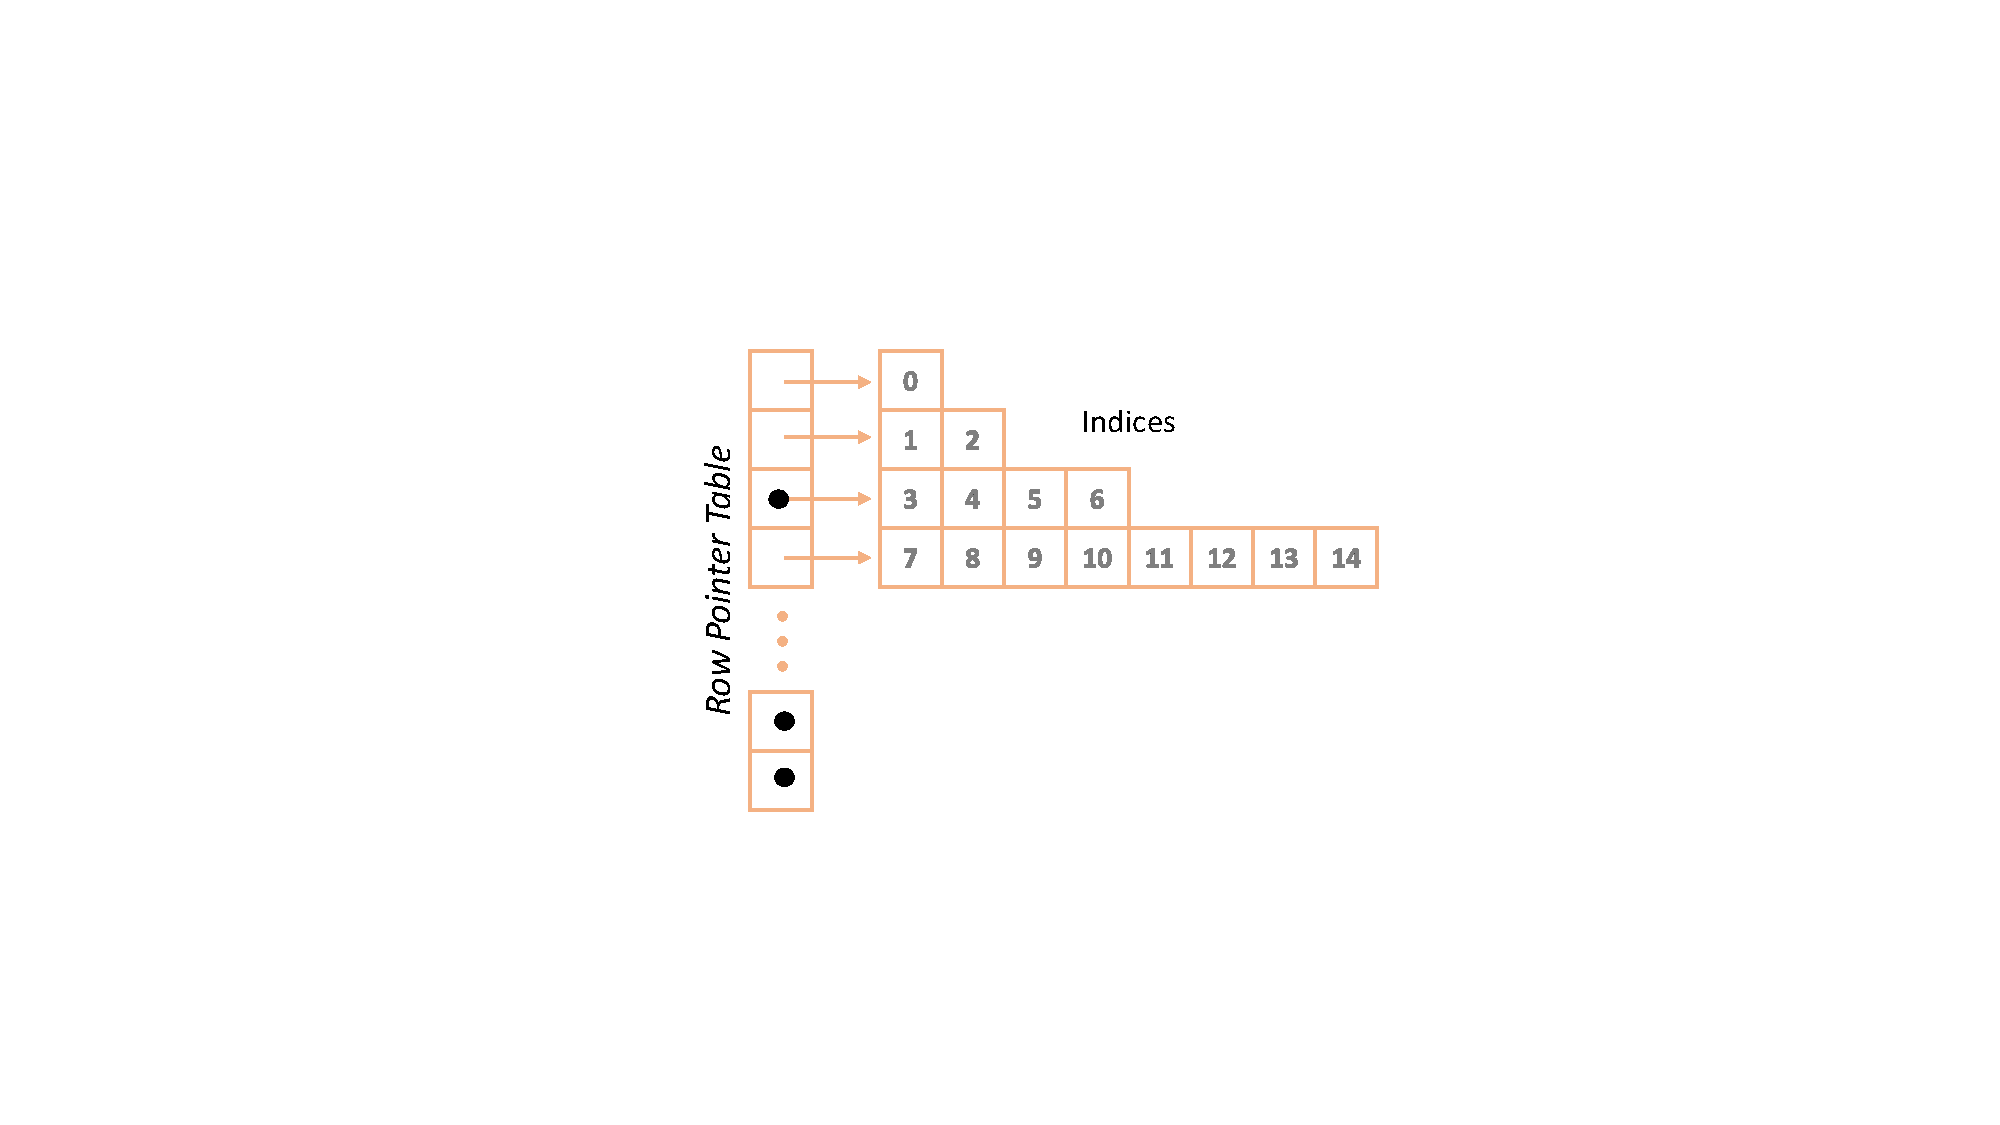
\includegraphics[clip,trim=0cm 3cm 0cm 3cm,width=1.00\textwidth,page=1]{../Pictures/bsa.pdf}
}
\caption{The Binary Sparse Array. A (vertical fixed-size) table allows access to each row. The rows
are size $1$ for the first, size $2$ for the second, size $4$ for third i.e. for row $k$ it's size is $2^{k}$.}
\label{fig:bsa1}
\end{figure}

However, the space allocation for each row is only done as-and-when
required. After creating an empty BSA, and inserting values into index
two and $12$, then only rows one and three will have been allocated,
as shown in Figure~\ref{fig:bsa2}.
\begin{figure}[ht]
\centering{
\includegraphics[clip,trim=0cm 3cm 0cm 3cm,width=1.00\textwidth,page=2]{../Pictures/bsa.pdf}
}
\caption{A Binary Sparse Array, showing values inserted into index $2$ and $12$ (shaded cells).
Other rows are currently unallocated.}
\label{fig:bsa2}
\end{figure}

\noindent If the only element in a row is deleted, then the entire row is freed up, as shown
in Figure~\ref{fig:bsa3} where the last element in row three is removed (index $12$).
\begin{figure}[ht]
\centering{
\includegraphics[clip,trim=0cm 3cm 0cm 3cm,width=1.00\textwidth,page=3]{../Pictures/bsa.pdf}
}
\caption{Deletion in a BSA can result in entire rows being freed up.}
\label{fig:bsa3}
\end{figure}


\begin{exercise}
Write an ADT to implement the \verb^bsa.h^ interface given.  Write the
source files \verb^Alloc/specific.h^ and \verb^Alloc/alloc.c^ such that
the driver files \verb^driver.c^,\verb^isfactorial.c^, \verb^sieve.c^ and \verb^fibmemo.c^
work correctly.  Ensure that this all works with my \verb^Makefile^
which {\bf must be} used {\bf unaltered}.  The basic operations are~:
\begin{verbatim}
bsa* bsa_init(void);
bool bsa_set(bsa* b, int indx, int d);
int* bsa_get(bsa* b, int indx);
bool bsa_delete(bsa* b, int indx);
int bsa_maxindex(bsa* b);
bool bsa_free(bsa* b);
\end{verbatim}

\noindent The function \verb^bsa_set()^ allows an integer to be written to a
particular index. If it is the first integer to be written into the row, then
the space for this will need to be allocated.

\noindent \verb^bsa_get()^ returns a pointer to the integer
stored in an index if it has been set, and \verb^NULL^ if it is a cell
that is not in use, hasn't been written to, deleted,  or past the end
the maximum index used.

\noindent The functions \verb^bsa_delete()^ `removes' an integer from an index
(maybe setting a Boolean flag to show if it's in use or not), and
if it was the only cell being used on that row, the entire row is freed.

\noindent Additional functionality includes~:
\begin{verbatim}
bool bsa_tostring(bsa* b, char* str);
void bsa_foreach(void (*func)(int* p, int* n), bsa* b, int* acc);
\end{verbatim}

\noindent \verb^bsa_tostring()^ allows a character based version of the BSA to be produced
with each row inside \verb^{}^ brackets. The function \verb^bsa_foreach^
allows a user-defined function to be passed which is performed on each
element in turn.

\begin{itemize}

\item The row pointer table is of a fixed size, and never gets deleted
until the final call to \verb^bsa_free()^.

\item You will never use \verb^realloc^ for the BSA - rows are created
as required using e.g. \verb^calloc()^ of a fixed size, and freed as
required.

\item Do not use the maths library in this assignment (my Makefile doesn't) -
use bit manipulation if required rather than e.g. \verb^log2()^.

\item Even if you don't get all the functions to work correctly, make
sure the code still compiles by writing `dummy' functions as placeholders,
even if some of the assertions fail.

\end{itemize}

\noindent {\bf This is worth $90\%$ of the marks.}
\vspace*{1ex}

\noindent
The manner in which you've been asked to implement the functionality above is {\bf very}
specific. However, exactly the same functionality (getting/setting etc.) could be implemented
in very different ways (linked lists, 1D dynamic arrays, trees, hashing etc.).
As an extension, write a `rival' version to implement
the core functionality of these functions without it necessarily being a BSA.
This should still ensure that \verb^fibmemo^, \verb^sieve^ and
\verb^isfactorial^ can be compiled against it. This means you
can ignore \verb^bsa_tostring()^ since this gives something very
specific to the `shape' of the BSA data structure.  Again, use an
unchanged version of my Makefile to achieve this.  These files will be
\verb^Extension/specific.h^ and \verb^Extension/extension.c^.

If you do this, submit \verb^extension.txt^ which details what you
have done, the motivation for it, and how well it works in practice (or
not), and comparing it with the original BSA.
This discussion (a few hundred words at most) is as (if not more)
important than the code itself.

\noindent {\bf This worth $10\%$ of the marks.}

\end{exercise}
